%\documentclass[jou]{apa6}
\documentclass[11pt]{article}
\usepackage{ucs}
\usepackage[utf8x]{inputenc}
\usepackage{changepage}
\usepackage{graphicx}
\usepackage{amsmath}
\usepackage{gensymb}
\usepackage{amssymb}
\usepackage{enumerate}
\usepackage{tabularx}
\usepackage{lipsum}
\usepackage{hyperref}
\usepackage{fancyvrb}

\oddsidemargin 0.0in
\evensidemargin 0.0in
\textwidth 6.27in
\headheight 1.0in
\topmargin -0.1in
\headheight 0.0in
\headsep 0.0in
\textheight 9.0in

\usepackage{xcolor}

\setlength\parindent{0pt}

\newenvironment{myenv}{\begin{adjustwidth}{0.4in}{0.4in}}{\end{adjustwidth}}
\renewcommand{\abstractname}{Anotācija}
\renewcommand\refname{Atsauces}



\newcounter{alphnum}
\newenvironment{alphlist}{\begin{list}{(\Alph{alphnum})}{\usecounter{alphnum}\setlength{\leftmargin}{2.5em}} \rm}{\end{list}}


%16.3-6

\makeatletter
\let\saved@bibitem\@bibitem
\makeatother

\usepackage{bibentry}



\begin{document}
\thispagestyle{empty}


\begin{center}
{\Large C++ Exercise 4: Matrix Operations}
\end{center}

\begin{abstract}
This exercise covers polymorphism, function overloading as well as operator
overloading, raising domain-specific exceptions or error conditions.
%% Example is about adding/subtracting/multiplying/dividing rational numbers (specific class to store them in canonic way)
%% https://softwareengineering.stackexchange.com/questions/149555/difference-between-immutable-and-const
%% Our rational numbers are "immutable"
\end{abstract}


%{\bf Deadline:} Friday, October 2, 2020 by 23:59:59 EEST Timezone.\\ 
{\bf How to submit:} Check your code into your GitHub repository, the default {\tt master} branch, 
tag it as {\tt ex04submit} (all lowercase, no dashes).\\
{\bf Grading:} This exercise is worth 30\textperthousand (or $3\%$) of the total grade.

%\vspace{10pt}
%{\small
%Three friends Zack, Quentin and Ralf want to calculate three arithmetic operations on matrices (addition, 
%subtraction and multiplication). They care about three different number sets respectively: 
%integers ($\mathbb{Z}$ represented by {\tt int} in C++), 
%rational numbers ($\mathbb{Q}$ represented by a custom class {\tt ds\textunderscore{}course::Ratio} 
%that will be covered and fully implemented in the class) and real numbers ($\mathtt{R}$ represented by {\tt double} in C++). 
%}

\vspace{10pt}
Develop a software that receives an input file containing
two rectangular matrices (in our math expressions we denote them by $A$ and $B$ respectively). 
Every matrix first displays its type ({\tt MZ}, {\tt MQ} or {\tt MR}), 
its dimensions (positive integers: row number $m$, column number $n$), followed by exactly $m \cdot n$ numbers
of the respective type. Both matrices are of the same type.

After that it receives an operation name ({\tt ADD}, {\tt SUB} or {\tt MUL}) and 
writes the resulting matrix to the standard output.
If matrix sizes do not allow the operation to be performed, 
throw {\tt std::out\textunderscore{}of\textunderscore{}range}. 

{\bf Valid matrix operations:} Assume that there is a matrix $A$ of size $m_1 \times n_1$ and
a matrix $B$ of size $m_2 \times n_2$:
\begin{enumerate}[(A)] 
\item
$C = A+B$ (operation {\tt ADD}) is doable iff $m_1 = m_2$ and $n_1 = n_2$ (both sizes match).
The elements $(c_{ij})$ of $C$ are defined as $c_{ij} = a_{ij} + b_{ij}$. 
\item 
$C = A-B$ (operation {\tt SUB}) is doable iff $m_1 = m_2$ and $n_1 = n_2$ (both sizes match).
The elements $(c_{ij})$ of $C$ are defined as $c_{ij} = a_{ij} - b_{ij}$.
\item 
$C = A \cdot B$ (operation {\tt MUL}) is doable iff $n_1 = m_2$ (the number of colums in the 
matrix to the left equals the number of rows in the matrix to the right). 
The elements $(c_{ij})$ of $C$ are defined as
$$c_{ij} = \sum\limits_{k=1}^{n_1} a_{ik}\cdot b_{kj},$$
kur $i \in \{ 1,\ldots,m_1\}$ un $j \in \{ 1,\ldots,n_2\}$.
\end{enumerate}



\vspace{10pt}
{\bf Input}

The first line contains abbreviation {\tt MZ}, {\tt MQ} and {\tt MR} followed by number of 
rows {\tt m} and the number of columns {\tt n} (two positive integers).  
After that there are $m \cdot n$ numbers (integers, rationals written with a 
forward slash {\tt p/q} or reals \textendash{} double type numbers). 

\vspace{10pt}
{\bf Output}

The output is either the result matrix (of the same type as the two input matrices). 
It shows type (MZ, MQ or MR) on the first line, also the count of rows and columns. 
After that it shows all the matrix elements - separated by spaces, line by line. 
If there was an exception, print just the exception name
{\tt out\textunderscore{}of\textunderscore{}range}.



\vspace{10pt}
{\bf Limitations}

\begin{itemize}
\item Any matrix in the input file has the number of rows and the 
number of columns between $1$ and $256$ (thus the largest matrix can be
$256 \times 256$).
\item Integer arithmetic when adding, subtracting or computing sums like 
$a_{i1}b_{1j} + \ldots$ should not overflow the size of {\tt int} register. 
(Namely, you should not worry about the order in which you add numbers themselves
or their products.)
\item The same assumption can be made about the rationals (class {\tt Ratio}) as
well as reals: You can add them in any order you want. The input data will not 
deliberately cause large rounding errors as in this example:
$$1000000000 + 0.00001 - 1000000000.$$
\item All the rational numbers (both input and output) are in the reduced form ($\operatorname{gcd}(p,q)=1$), 
denominators are always positive. For example, the rational number $-0.5$ is always input and output
as $\mathtt{-1/2}$ (and never as $\mathtt{-6/3}$ or $\mathtt{1/-2}$). 
\item Rational numbers that happen to be integers still have denominator $1$ explicitly written. 
For example, the rational number $17$ in {\tt MQ} matrices is always written as $\mathtt{17/1}$.
\item All matrices in the input will be presented correctly, but sometimes the operations may be
impossible.
\end{itemize}


\vspace{10pt}
{\bf Notes on Strassen's Algorithm}

It could be tempting to consider Strassen's Algorithm for multiplying matrices that 
are sufficiently large (the number of arithmetic 
operations would be about $O(n^{2.8074})$ instead of  $O(n^3)$). 
On the other hand, it is likely require
very large matrices (at least a few thousand by a few
thousand) to see any savings when compared with the school algorithm for 
matrix multiplication. See \url{https://bit.ly/3jblOWX} for more discussion on this.

We will have other examples in this course where algorithm can be designed 
to be more efficient. You could try to implement Strassen's algorithm, 
if the current task seems too straightforward.




\vspace{10pt}
\begin{tabular}{@{}ll@{}}
\begin{minipage}[t]{0.49\columnwidth}
Sample input {\bf test01in.txt}:
\begin{verbatim}
MZ 3 3
2 -6 8
10 6 -1
-4 -5 0 
MZ 3 4
2 -6 -10 -1
6 -5 10 0
9 4 5 -4
MUL
\end{verbatim}
\end{minipage} 
&
\begin{minipage}[t]{0.49\columnwidth}
Expected output {\bf test01expected.txt}:
\begin{verbatim}
MZ 3 4
40 50 -40 -34
47 -94 -45 -6
-38 49 -10 4
\end{verbatim}
\end{minipage} 
\end{tabular}

\vspace{10pt}
\begin{tabular}{@{}ll@{}}
\begin{minipage}[t]{0.49\columnwidth}
Sample input {\bf test02in.txt}:
\begin{verbatim}
MQ 2 2
0/1 6/5
-5/9 -1/1
MQ 2 2
-7/4 3/10
5/9 1/8
ADD
\end{verbatim}
\end{minipage} 
&
\begin{minipage}[t]{0.49\columnwidth}
Expected output {\bf test02expected.txt}:
\begin{verbatim}
MQ 2 2
-7/4 3/2
0 -7/8
\end{verbatim}
\end{minipage} 
\end{tabular}

\vspace{10pt}
\begin{tabular}{@{}ll@{}}
\begin{minipage}[t]{0.49\columnwidth}
Sample input {\bf test03in.txt}:
\begin{verbatim}
MR 2 3
1 0.3 0
0 0.7 1
MR 2 2
1.0 0
0 1.0
MUL
\end{verbatim}
\end{minipage} 
&
\begin{minipage}[t]{0.49\columnwidth}
Expected output {\bf test03expected.txt}:
\begin{verbatim}
out_of_range
\end{verbatim}
\end{minipage} 
\end{tabular}




\vspace{10pt}
{\bf Implementation Details}

\begin{enumerate}
\item Implement files {\tt Ratio.h} (optionally also {\tt Ratio.cpp}), 
{\tt Matrix.h} (optionally also {\tt Matrix.cpp}) and also 
{\tt MatricMain.cpp}.
(You may find that header-only implementation is the most easy to build on most
C++ compilers, but using CPP files isfine.) 
\item It is recommended to implement  
the following UML diagram using operator overloading
(see Figure~\ref{fig:ex04-uml-diagram}).\\
{\bf Note:} Just as in previous tasks, your main concern should be passing the
Standard Input/Output testcases, since your grade for EX04 only depends on these. 
Still, we strongly recommend to follow the UML diagram since 
the following exercise (EX05) will assume that the UML diagram is implemented;
it will build on top of these overloaded operators and interfaces. 
\end{enumerate}

\begin{figure}[!htb]
\center{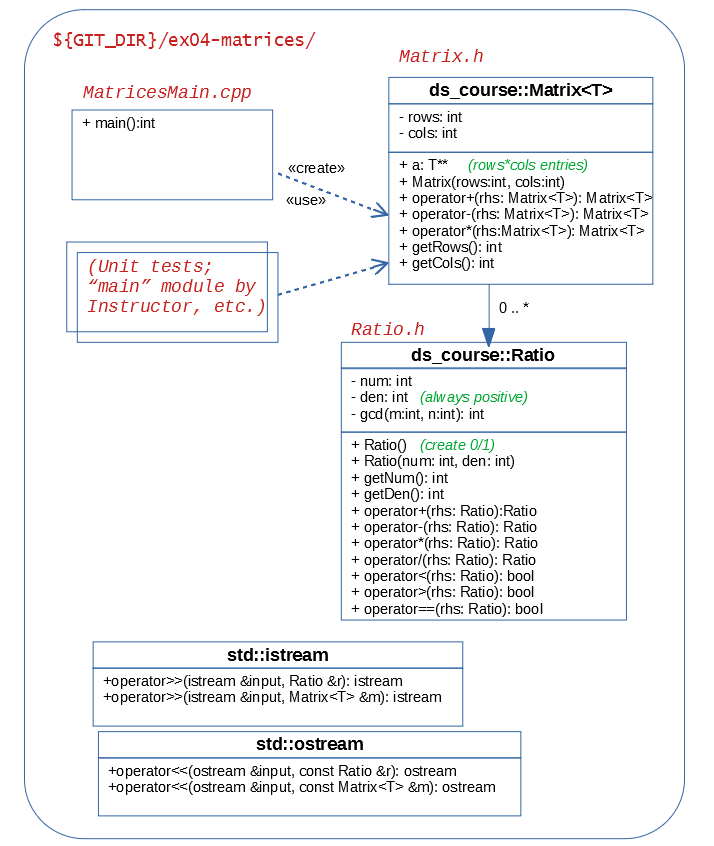
\includegraphics[width=6in]{ex04-uml-diagram.png}}
\caption{\label{fig:ex04-uml-diagram} Classes and functions suggested for EX04.}
\end{figure}





%% 
%% Sth.
%% 


%% External demo... 
%% Homogeneous coordinates in 2D - an example that paints SVG. 
%% It should be able to eat some transformation matrices, apply multiplication
%% Then it takes some figure (e.g. L-shape) - and arranges it somehow.


%% Some discussion why rational numbers should be made immutable (note that the 
%% https://introcs.cs.princeton.edu/java/92symbolic/Rational.java.html

%% https://en.wikipedia.org/wiki/Rep-tile
%% 

%% https://scicomp.stackexchange.com/questions/4666/what-is-the-criteria-for-switching-between-strassens-and-regular-matrix-multipl

%% https://github.com/saif86/Rational-Numbers---Operator-Overloading/blob/master/RationalNumber.h
%% https://github.com/saif86/Rational-Numbers---Operator-Overloading/blob/master/RationalNumber.cpp

\end{document}



